\section{Strojno ucenje}


\subsection{Problemski prostor, ocenjevanje znanja}

\subsection{Evalviranje hipotez}
Pomembni kriteriji:
\begin{itemize}[leftmargin=*,labelindent=0pt,labelwidth=0pt,itemsep=0pt,parsep=0pt,topsep=0pt]
    \item \textbf{konsistentnost} hipotez z primeri (ucnimi)
    \item \textbf{splosnost} (tocnost za nevidene primere)
    \item \textbf{razumljivost} hipotez
\end{itemize}
Ocenjevanje uspesnosti pri klasifikaciji na podlagi njihove \textbf{tocnosti}:\\
TP - true positive, FP - false positive, FN - false negative, TN - true negative
$$\text{Klasifikacijska tocnost}=\frac{TP+TN}{TP+TN+FP+FN}=\frac{TP+TN}{N}$$
Napaka 1. tipa = FP, napaka 2. tipa = FN
$$\text{Obcutljivost/senzitivnost}=TPR=\frac{TP}{TP+FN}$$

\subsection{Gradnja odlocitvenih dreves}
\textbf{Informacijski prispevek} $\text{Gain(A)}=I-I_{res}(A)$, I=H(C)
$$I_{\text{res}}=-\sum_{v_i\in A}p_{v_i}\sum_c p(c|v_i)\log_2p(c|v_i)$$
Za koliko se entropija zmanjsa po delitvi z Atributom A.\\
\textbf{Razmerje inofrmacijskega prispevka atributa A}:\\ 
$\text{IGR(A)}=\frac{\text{Gain(A)}}{\text{H(A)}}$\\


\subsubsection{TDIDT (Top down induction decision tree) algoritem}
Pozresen algoritem, ki \textbf{lokalno} izbira najbolsi atribut.\\
- kratkoviden algoritem

\subsubsection{Binarizacija atributov}
Aleternativa za resevanje problematike z vecvrednostnimi atributi:\\
Primer: barve $\in$ {rdeca, rumena, zelena, modra}\\
Strategije, razbijemo v dve mnozici:\\
- {{rdeca}, {rumena, zelena, modra}}\\
- {{rdeca, rumena}, {zelena, modra}}\\
\textbf{Prednost}: manjse vejanje drevesa.



\subsection{Ucenje iz sumnih podatkov (rezanje)}
\green{tocnost t}...verjetnost pravilnosti klasifikacije\\
\green{napaka e} $\dots$ $1-t$\\
\green{relativna frekvenca} $p=\frac{n}{N}$\\
\green{m-ocena} $p=\frac{n + p_a * m}{N+m}$\\
$m \dots$ koliko zaupam apriorni verjetnosti\\
$p_a$ apriorna verjetnost (domenski ekspert lahko pove)\\
\green{Laplacova ocena verjetnosti} $p=\frac{n+1}{N+k}$\\
k...stevilo vseh moznih razredov\\
\subsubsection{REP (reduced error prunning)} 
Dela dobro ce imamo veliko rezalno mnozico.\\
Obicajno uporabljamo relativno frekvenco za ocenjevanje verjetnosti.\\
$G(v)=\#\text{napak}_T-\#\text{napak}_v$\\
$G(v)\geq 0 \Rightarrow$ rezemo podrevo\\
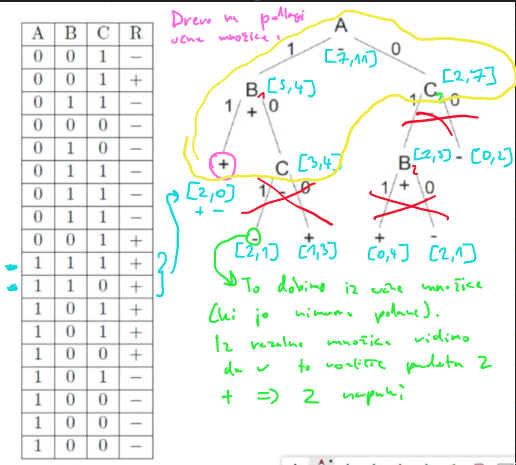
\includegraphics[width=6.5cm]{./images/rep.png}\\
$e(C)=3$\\
$e_T=2+3=5$\\
$G(C)=5-3=2\geq0 \rightarrow \text{rezemo}$
\subsubsection{MEP (Minimal Error Prunning)}
e...staticna napaka,E...vzvratna napaka,$e\leq E \rightarrow$ rezemo poddrevo\\
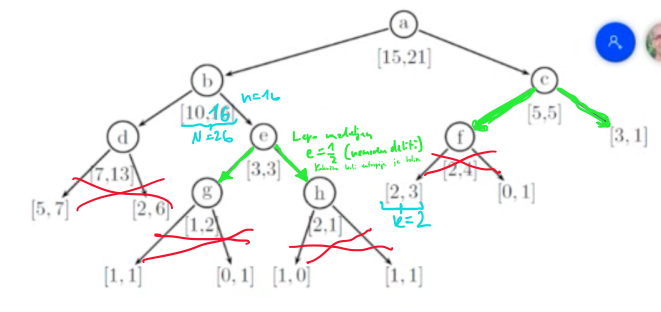
\includegraphics[width=6cm]{./images/mep.png}\\
(Laplace)\\
$e_L(d)=1-t=1-\frac{13+1}{20+2}=0.363$\\
$E_L(d)=12/20\cdot e_L(d_l) + 8/20\cdot e_L(d_d)= \frac{12}{20} \cdot(1-\frac{7+1}{12+2})+\frac{8}{20}(1-\frac{13+1}{20+2})$\\


\subsection{Ocenjevanje uspesnosti modelov}
\green{tocnost t} $\dots$ verjetnost pravilnosti klasifikacije\\
\green{Laplacova ocena verjetnosti} $p=\frac{n+1}{N+k}$\\
k...stevilo vseh moznih razredov\\
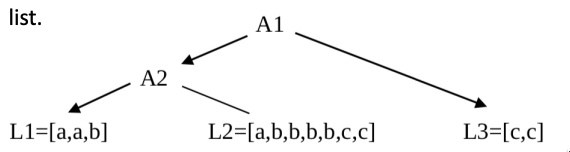
\includegraphics[width=6cm]{./images/drevo-laplace.png}\\
$t_{L1}=\frac{2+1}{3+3}=0.5$,
$t_{L2}=\frac{4+1}{7+3}=0.5$,
$t_{L3}=\frac{2+1}{2+3}=0.6$\\
tocnost drevesa: $t_D=3/12\cdot 0.5 + 7/12\cdot 0.5 + 2/12\cdot 0.6=0.5167$\\
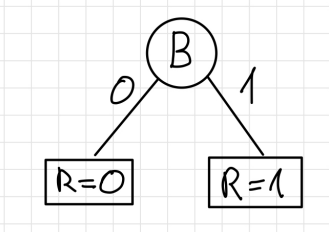
\includegraphics[width=6cm]{./images/klasifikacijska-napaka.png}\\
$e=1-(P(B=0)P(R=0|B=0)+P(B=1)P(R=1|B=1))$\\


\subsection{Obravnanva mankajocih atributov, navini Bayesov klasifikator}
\subsubsection{Naivni bayes}
Ce poznamo razred, kam klasificiramo ce nepoznamo atributov:
$$\text{Klasifikator: }\text{argmax}_{c\in C} P(c)\prod_{i=1}^n P(x_i|c)$$
$c\dots \text{razred}$, $x_i\dots \text{atributi}$\\
Verjetnost::
$$P(C=c|x_1,\dots,x_n)=\frac{P(C=c)P(X_1=x_i|C=c)P(X_2=x_j|C=c)\dots}{P(X_1=x_i)P(X_2=x_j)\dots}$$

\text{Primer moski}: $\text{visina}\geq175, \text{teza}\geq 65, \text{spol}=M$
$$
\begin{array}{|c|c|c|}
    \hline
    X\backslash Y   & \text{Razred A}      & \text{Razred B}\\
    \hline
    p_a           & P(A) = \frac{2}{3}    & P(B) = \frac{1}{3}\\
    \hline
    \text{spol}   & P(M|A) & P(M|B)\\
    \hline
    \text{visina} & P(V\geq 175|A) & P(V\geq 175 | B)\\
    \hline
    \text{teza} & P(T\geq 65|A) & P(T\geq 65| B)\\
    \hline
    P(y)\prod\limits_{i=1}^n P(x_i|y) & \dots & \dots\\
    \hline
\end{array}
$$

\subsubsection{Nomogragmi}
Ciljni razred $C=c_T$
$$X_{X_i=x_j}=\ln \left( \frac{P(X_i=x_j|C=c_T)}{P(X_i=x_j|C=\overline{c_T})} \right)$$

\subsection{K-najblizjih sosedov}
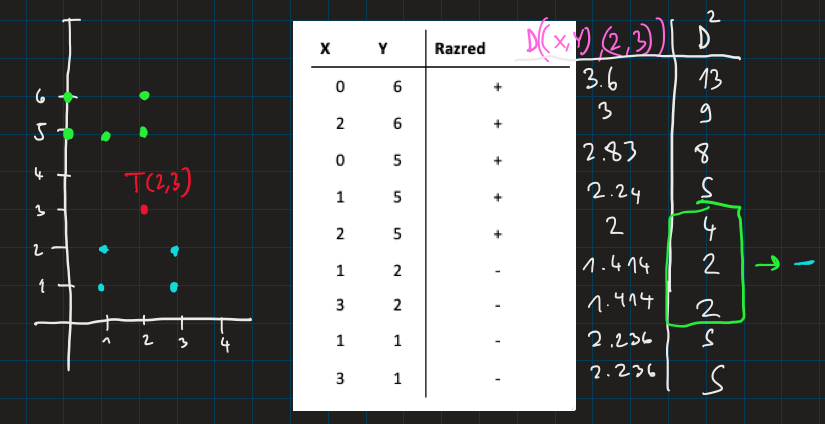
\includegraphics[width=6cm]{./images/knn.png}\\


\section{Vrste ucenja}
\subsection{Nadzorovano ucenje (supervised learning)}
\textbf{Ucni primeri so podani/oznaceni} kot \textbf{vrednosti vhodov in izhodov}.\\
$(\vec{x}_1,\vec{y}_1),(\vec{x}_2,\vec{y}_2),\dots,(\vec{x}_N,\vec{y}_N)$\\
$\vec{x}_i\dots$ atributi, $\vec{y}_i\dots$ ciljna spremenljivka\\
Locimo dve vrsti problemov:
% Create the list of problems with no margins
\begin{enumerate}[leftmargin=*,noitemsep,topsep=0pt,partopsep=0pt]
    \item \textbf{Klasifikacijski problemi} - $y_j$ \underline{diskretna} 
    \item \textbf{Regresijski problemi} - $y_j$ \underline{zvezna} 
\end{enumerate}

\subsubsection{Lokalno utezena regresija}
$$h(\vec{x}_?) = \frac{\sum\limits_{i=1}^k w_i\cdot f(\vec{x}_i)}{\sum\limits_{i=1}^k w_i}, \: w_i(d) ... \text{utez}$$
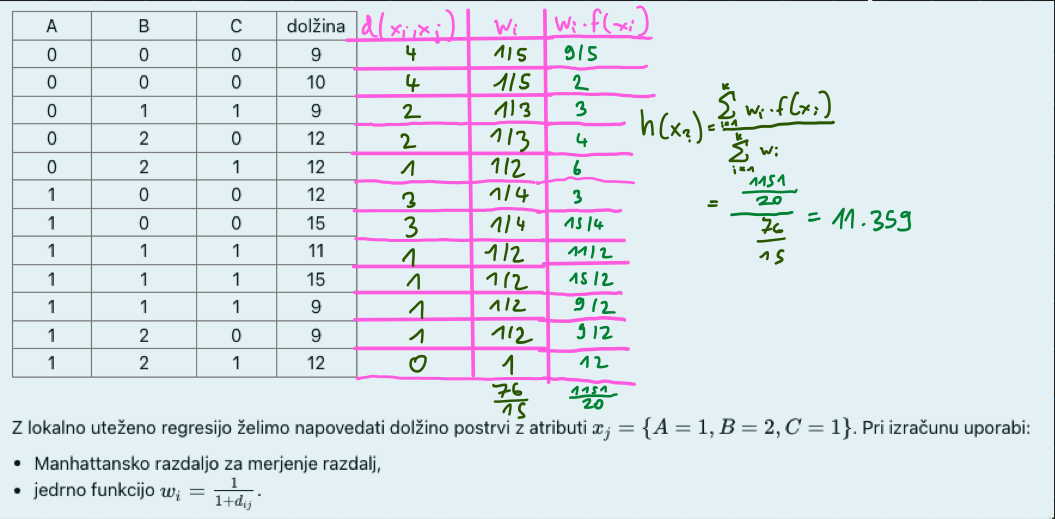
\includegraphics[width=7cm]{./images/lokalno-utezena-regresija.png}\\



\subsubsection{Regresijska drevesa}
Linearna regresija je poseben primer regresijskega drevesa.\\
V listih regresijskega drevesa vcasih napovemo kar povprecno vrednost.

\subsection{Nenadzorovano ucenje (unsupervised learning)}
\textbf{Ucni primeri niso oznaceni} (nimajo ciljne spremenljivke),
\textbf{ucimo se vzorcev v podatkih}, (npr. grucenje)

\subsubsection{Hierarhicno grucenje}
Poveze po podobnosti med primeri, primer zacne kot samostojna gruca, na koncu vsi primeri pripadajo eni gruci\\
\textbf{Dendrogram}: drevo, ki predstavlja grucenje.\\
\textbf{Single-linkage}: povezava med grucami je najkrajse razdalje med primeroma iz razlicnih gruc.\\
\textbf{Complete-linkage}: povezava med grucami je najdaljsa razdalja med primeroma iz razlicnih gruc.\\
\textbf{Average-linkage}: povezava med grucami je povprecna razdalja med primeroma iz razlicnih gruc.\\


\subsubsection{K-means}
1. V prostor dodamo k centroidov, ki predstavljajo gruce.\\
2. Izracunamo ketri centroid je najblizji vsakemu primeru.\\
3. Izracunamo nove centre gruc = $\frac{1}{|G|}\sum\limits_{i\in G} x_i$\\
4. Ponovimo korake 2 in 3 dokler se centri ne premaknejo.\\

\subsection{Spodbujevalno ucenje - reinforcement learning}
Inteligentni agent se uci iz zaporedja \textbf{nagrad} in \textbf{kazni}

\subsection{Ocenjevanje ucenja}

\subsubsection{Precno preverjanje}
Poseben primer \textbf{veckratnega ucenja} in testiranja\\
\textbf{k-kratno precno preverjanje}
\begin{itemize}[leftmargin=*,noitemsep,topsep=0pt,partopsep=0pt]
    \item celo ucno mnozico razbij na k disjunktnih podmnozic
    \item za vsako od k podmnozic:
    \begin{itemize}[leftmargin=*,noitemsep,topsep=0pt,partopsep=0pt]
        \item uporabi \textbf{mnozico} kot \textbf{testno mnozico}
        \item uporabi \textbf{preostalih k-1} mnozic kot \textbf{ucno mnozico}
    \end{itemize}
    \item povpreci dobljenih k ocen tocnosti v koncno oceno
\end{itemize}
Pri precnem preverjanju uporabimo vse podatke za testiranje in vse za ucenje\\
Metoda \textbf{leave one out} je poseben primer precnega preverjanja\\
Imamo dve hipotezi A in B. Izkase se, da A bolje napoveduje na ucnih podatkih
B pa na testnih. Potem je B verjetno boljsa hipoteza.
